% 119-17(119쪽) — 삼차함수 y=f(x) 와 일차함수 y=g(x) 의 그래프 · 두 그래프가 x=1 과 x=3 에서 만나 그 사이를 색칠한 그림. 스캔 화질이 낮아 TikZ 로 다시 그림.
% 원문에 있는 것만: 눈금 1 · 3 · 라벨 O, x, y, y=f(x), y=g(x) · x=1, x=3 안내 파선 · 색칠한 부분. 넓이 4 는 글로만 주어지고 그림에는 없다.
% 곡선·직선의 식은 원문에 없다. 원문 모양(x=1 과 x=3 에서 만나고 그보다 왼쪽에서 한 번 더 만나는 삼차함수)만 맞춘 보조식이며 눈금이 없어 값을 잴 수 없다.
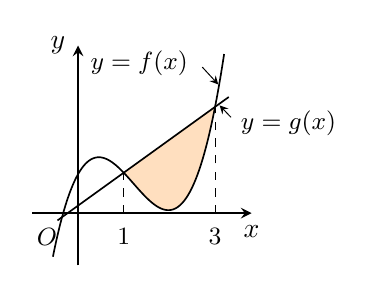
\begin{tikzpicture}[x=0.58cm, y=0.38cm, line width=0.5pt]
  % 색칠한 부분(1<=x<=3 · 위는 직선 y=g(x), 아래는 곡선 y=f(x))
  \fill[orange!25] plot[domain=1:3, samples=40] (\x, {1.1*(\x)+0.25}) -- plot[domain=3:1, samples=70, smooth] (\x, {(\x)*(\x)*(\x)-3.65*(\x)*(\x)+2.7*(\x)+1.3}) -- cycle;
  % 축
  \draw[->, >=stealth, line width=0.7pt] (-1.0,0) -- (3.8,0) node[below=1pt] {$x$};
  \draw[->, >=stealth, line width=0.7pt] (0,-1.75) -- (0,5.6) node[left=1pt] {$y$};
  % 안내 파선(원문)
  \draw[dashed, line width=0.35pt] (1,0) -- (1,1.35);
  \draw[dashed, line width=0.35pt] (3,0) -- (3,3.55);
  % 그래프
  \draw[line width=0.6pt, domain=-0.55:3.2, samples=160, smooth] plot (\x, {(\x)*(\x)*(\x)-3.65*(\x)*(\x)+2.7*(\x)+1.3});
  \draw[line width=0.6pt] (-0.45,-0.245) -- (3.3,3.88);
  % 라벨(원문 자리 그대로)
  \node[below=2pt, font=\small] at (-0.68,0) {$\pt{O}$};
  \node[below=2pt, font=\small] at (1,0) {$1$};
  \node[below=2pt, font=\small] at (3,0) {$3$};
  \node[anchor=east, font=\small] at (2.62,5.0) {$y=f(x)$};
  \draw[->, >=stealth, line width=0.35pt] (2.72,4.88) -- (3.07,4.3);
  \node[anchor=west, font=\small] at (3.35,3.0) {$y=g(x)$};
  \draw[->, >=stealth, line width=0.35pt] (3.35,3.2) -- (3.1,3.6);
\end{tikzpicture}
